% Created 2021-09-11 Sat 09:36
% Intended LaTeX compiler: xelatex
\documentclass[letterpaper]{article}
\usepackage{graphicx}
\usepackage{grffile}
\usepackage{longtable}
\usepackage{wrapfig}
\usepackage{rotating}
\usepackage[normalem]{ulem}
\usepackage{amsmath}
\usepackage{textcomp}
\usepackage{amssymb}
\usepackage{capt-of}
\usepackage{hyperref}
\usepackage[margin=1in]{geometry}
\usepackage{fontspec}
\usepackage{indentfirst}
\setmainfont[ItalicFont = LiberationSans-Italic, BoldFont = LiberationSans-Bold, BoldItalicFont = LiberationSans-BoldItalic]{LiberationSans}
\newfontfamily\NHLight[ItalicFont = LiberationSansNarrow-Italic, BoldFont       = LiberationSansNarrow-Bold, BoldItalicFont = LiberationSansNarrow-BoldItalic]{LiberationSansNarrow}
\newcommand\textrmlf[1]{{\NHLight#1}}
\newcommand\textitlf[1]{{\NHLight\itshape#1}}
\let\textbflf\textrm
\newcommand\textulf[1]{{\NHLight\bfseries#1}}
\newcommand\textuitlf[1]{{\NHLight\bfseries\itshape#1}}
\usepackage{fancyhdr}
\pagestyle{fancy}
\usepackage{titlesec}
\usepackage{titling}
\makeatletter
\lhead{\textbf{\@title}}
\makeatother
\rhead{\textrmlf{Compiled} \today}
\lfoot{\theauthor\ \textbullet \ \textbf{2021-2022}}
\cfoot{}
\rfoot{\textrmlf{Page} \thepage}
\titleformat{\section} {\Large} {\textrmlf{\thesection} {|}} {0.3em} {\textbf}
\titleformat{\subsection} {\large} {\textrmlf{\thesubsection} {|}} {0.2em} {\textbf}
\titleformat{\subsubsection} {\large} {\textrmlf{\thesubsubsection} {|}} {0.1em} {\textbf}
\setlength{\parskip}{0.45em}
\renewcommand\maketitle{}
\author{Exr0n}
\date{\today}
\title{Problems to Practice \LaTeX{}}
\hypersetup{
 pdfauthor={Exr0n},
 pdftitle={Problems to Practice \LaTeX{}},
 pdfkeywords={},
 pdfsubject={},
 pdfcreator={Emacs 27.2 (Org mode 9.4.4)}, 
 pdflang={English}}
\begin{document}

\maketitle
\#ret

\section{Square roots of \(i\)}
\label{sec:org3e43337}
\href{20math530retSquareRootsi.pdf.org}{20math530retSquareRootsi.pdf}
Didn't figure it out. How did I get \(a = \pm\frac{\sqrt{2}i}{2}\)??

\section{Cross product}
\label{sec:orgba1df6b}
\begin{quote}
Find the cross product of
\(\begin{pmatrix}1\\3\\0\end{pmatrix}\times\begin{pmatrix}2\\2\\-1\end{pmatrix}\)
\end{quote}

$\backslash$[
\begin{split}
\Rightarrow&\left|\begin{matrix}i&j&k\\1&3&0\\2&2&-1\end{matrix}\right|\\
\Rightarrow&i\left|\begin{matrix}3&0\\2&-1\end{matrix}\right|
+j\left|\begin{matrix}0&1\\-1&2\end{matrix}\right|
+k\left|\begin{matrix}1&3\\2&2\end{matrix}\right|\\
\Rightarrow& -3i + 1j -4k\\
\Rightarrow& \begin{bmatrix}-3\\1\\-4\end{bmatrix}
\end{split}
$\backslash$]

\section{Read Chapter 1.B}
\label{sec:orgb1997e5}
\subsection{Vector Space Addition/scalarmult}
\label{sec:org213f9a6}
\begin{itemize}
\item Every pair of elements is in \(V\) can be added together to form
another element in \(V\) (closed)
\item \textbf{A scalar is anything in \(F\), which means it might be complex!} \#\#\#
Vector space definition
\item communativity(!): \(u +v = v+u. \forall u, v \in V\)
\item associativity:
\((u+v)+w = u+(v+w) and (ab)v = a(bv). \forall u, v, w \in V. \forall a, b \in F\)
\item additive identity: \(\exists 0\in V \mid v + 0 = v. \forall v \in V\)
\item Additive inverse
\item Multiplicative identity (denoted \(1\))
\item distributive property (both front and back) A vector space depneds on
\(F\) so \(V\) is a \textbf{vector space over \(F\)} \#\#\# Vector spaces with
other sets? \(F^S\)
\item \(F^S\) is the set of functions from \(S\) to \(F\)

\begin{itemize}
\item meaning that it's all functions whose domains are subsets of \(S\)
and ranges are subsets of \(F\)?
\end{itemize}

\item addition \(f, g \in F^S, x \in F: (f + g)(x) = f(x)+g(x)\)
\item multiplication: \(\lambda \in F\) and
\(f \in F^S : \lambda F \in F^S = (\lambda f)(x) = \lambda f(x)\)
\item functions can be elements in fields or something?
\item lists are just functions on a set of numbers..?
\item subtraction (additive inverses and identity are unique)
\item \textbf{When you see \(xy\), one of them has to be a vector because there is
no scalar scalar multiplication defined} \#\# Show that
\(a\bullet b = |a||b|cos\theta\) Suppose
\(a = \begin{bmatrix}x\\y\end{bmatrix}\) and
\(b = \begin{bmatrix}w\\z\end{bmatrix}\). We have
\(a\bullet b = a^T\cdot b = \begin{bmatrix}x&y\end{bmatrix} \begin{bmatrix}w\\z\end{bmatrix} = xw+yz\).
We need an expresion for \(\theta\):
\begin{center}
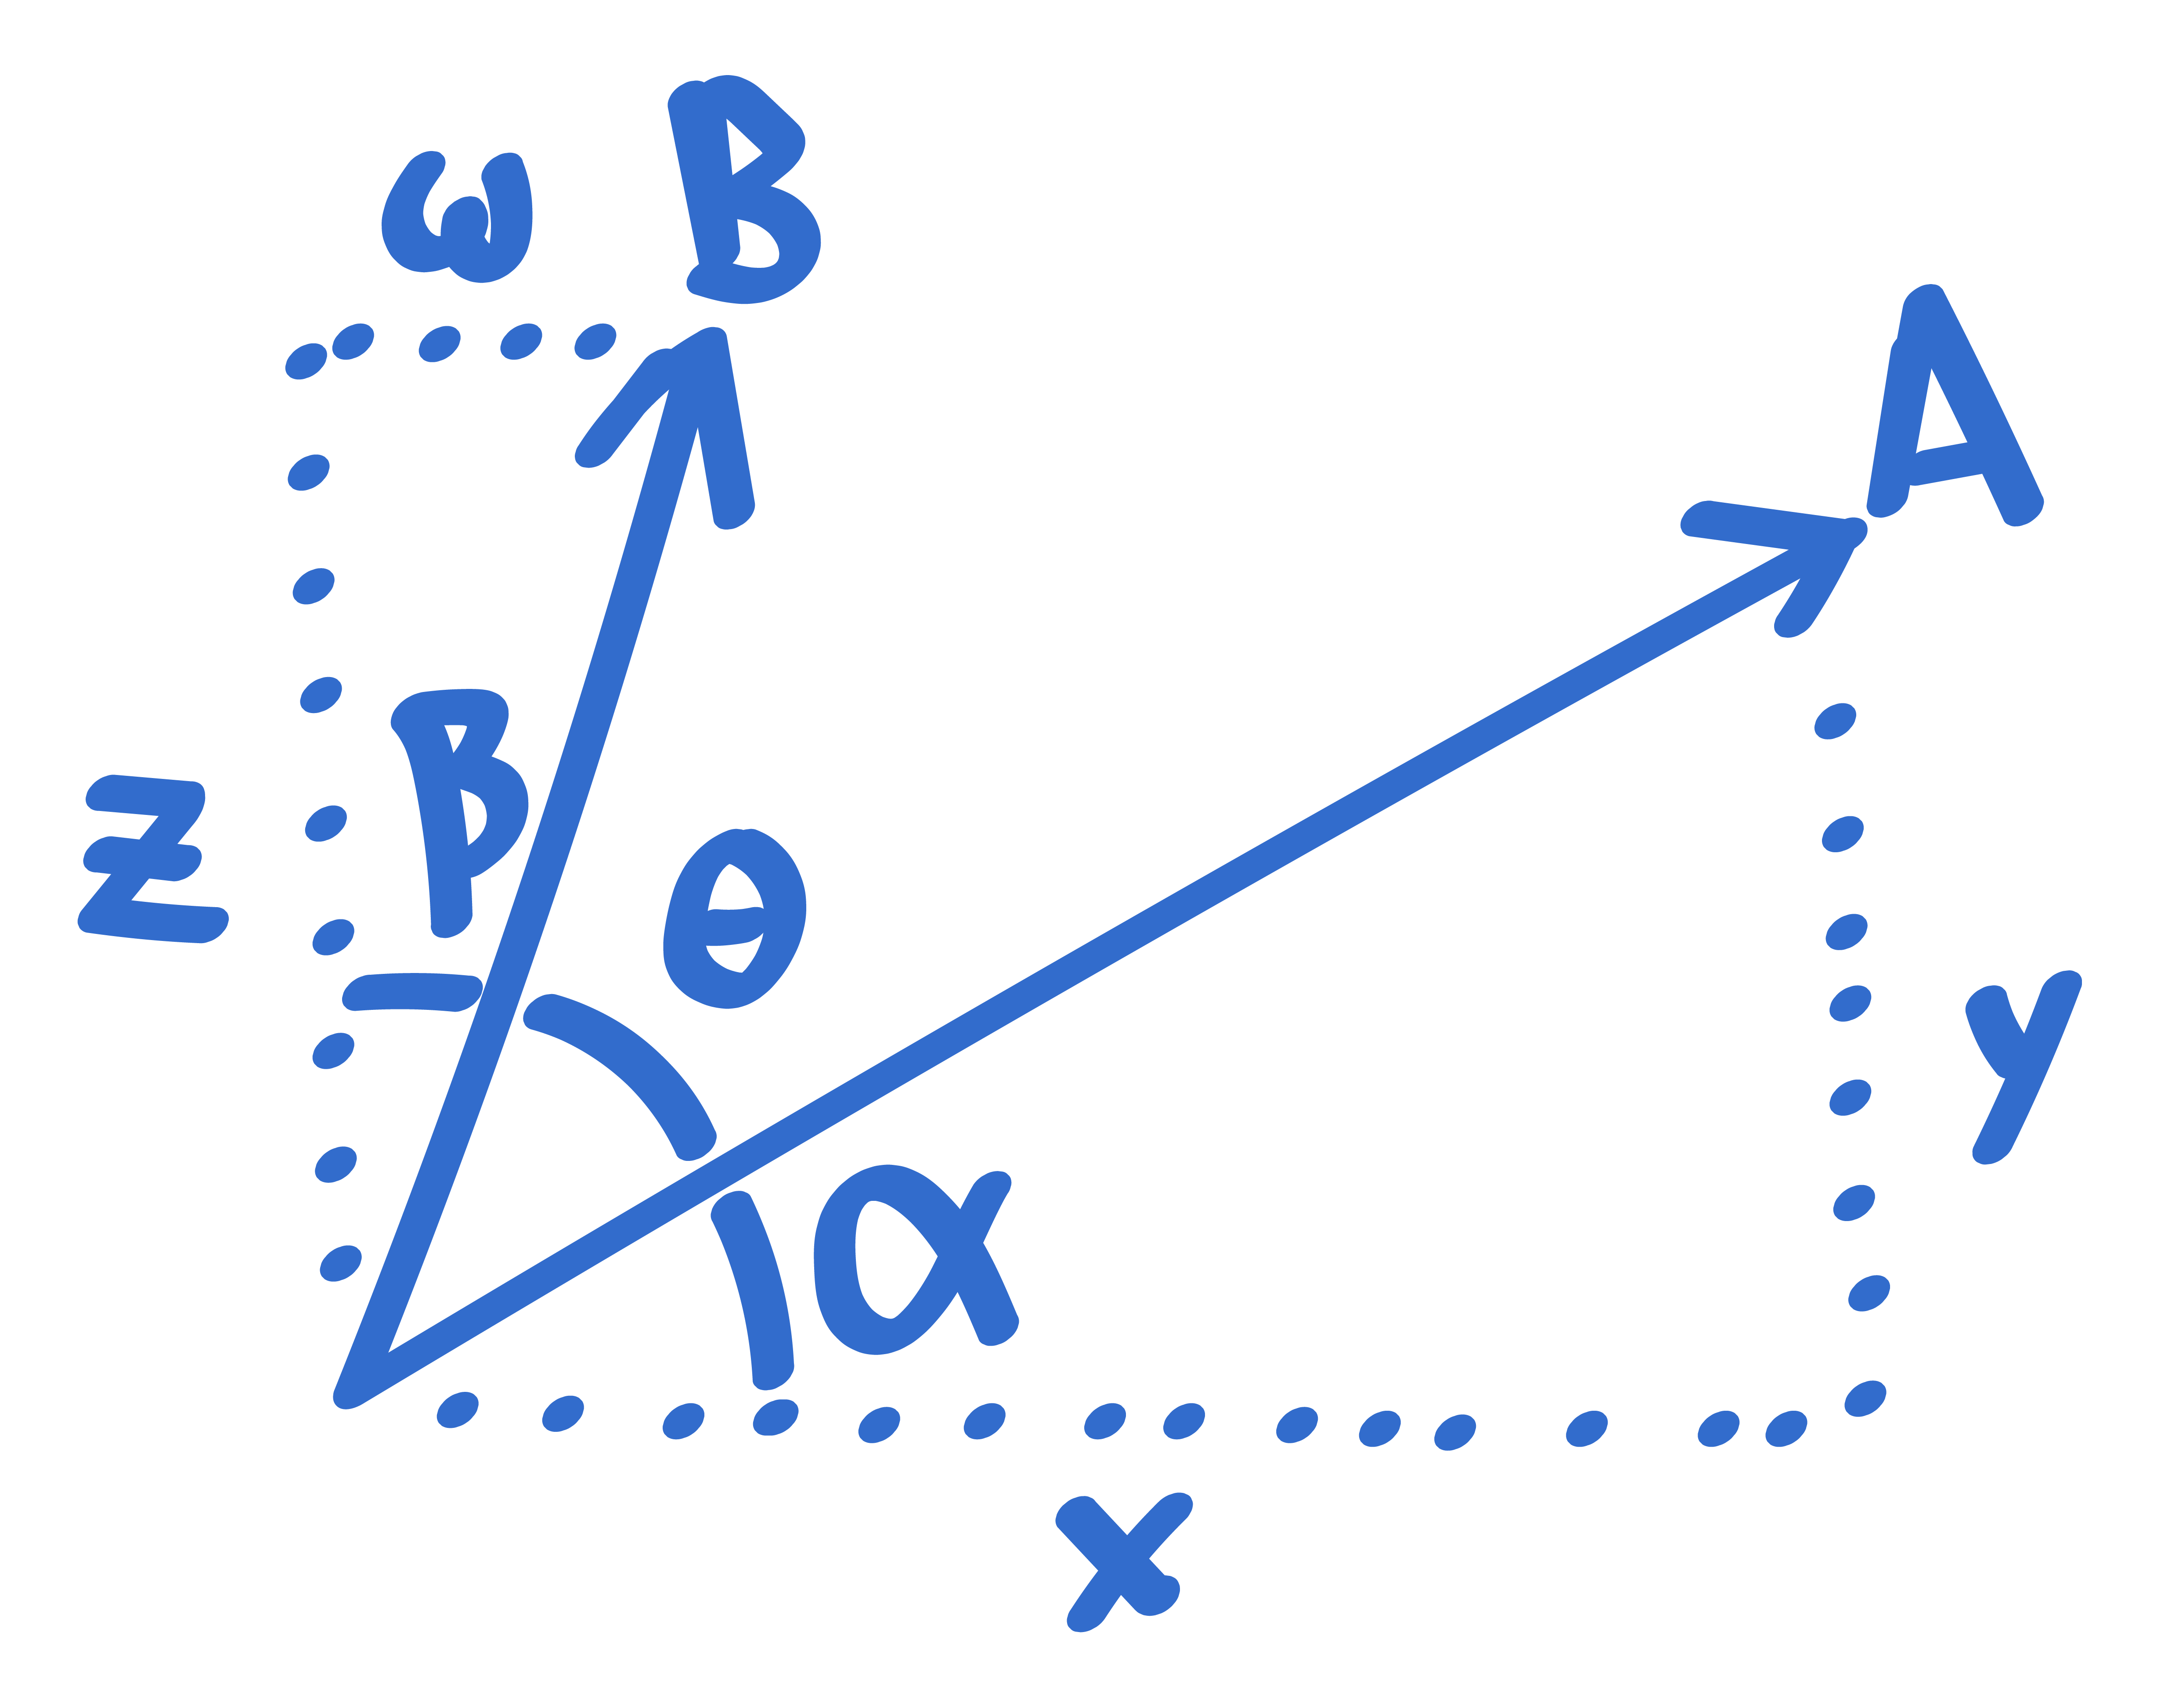
\includegraphics[width=.9\linewidth]{KBe20math530retDotProductProofFig.png}
\end{center} As seen in the diagram,
\(\theta = \frac{\pi}{2} - \alpha - \beta\). Finally: $\backslash$[
\begin{split}
|A||B|cos\theta &= |A||B| cos\left(\frac{\pi}{2}-\alpha-\beta\right)\\
&= |A||B| sin(\alpha + \beta)\\
&= |A||B| \left(sin\alpha\ cos\beta + cos\alpha\ sin\beta\right)\\
&= |A||B| \left(\left(\frac{y}{|A|}\right)\left(\frac{z}{|B|}\right)+\left(\frac{x}{|A|}\right)\left(\frac{w}{|B|}\right)\right)\\
&= |A||B| \left(\frac{yz}{|A||B|}+\frac{xw}{|A||B|}\right)\\
&= yz+wz\\
&= xw+yz
\end{split}
$\backslash$]
\end{itemize}

\section{Epilogue}
\label{sec:orgf8d80dc}
That was two hours\ldots{} I'll save the proving integers mod 3 are a field
for later. \#todo-exr0n

\noindent\rule{\textwidth}{0.5pt}
\end{document}
